\documentclass[pdftex,english,oribibl]{llncs}

%% Spracheinstellungen laden
\usepackage[english]{babel}

%% Schriftart in der Ausgabe/Eingabe
\usepackage[T1]{fontenc}
\usepackage{textcomp}
\usepackage[latin1]{inputenc}

%% Zitate
\usepackage[numbers]{natbib}
\bibliographystyle{abbrvnat}
%\bibliographystyle{dinat}
%\bibliographystyle{plainnat}
%\bibliographystyle{splncs}
%% Similar to option "sectionbib" but \refname instead of \bibname
\makeatletter
\renewcommand\bibsection{\section*{\refname\@mkboth{\MakeUppercase{\refname}}{\MakeUppercase{\refname}}}}
\makeatother

%% Index
%\usepackage{makeidx}
%\makeindex

%% PDF Einstellungen
% muss nach natbib geladen werden!
\usepackage{nameref}
\usepackage{varioref}
\usepackage[pdfusetitle,pdftex,colorlinks]{hyperref}
\hypersetup{pdfborder={0 0 0}}
\hypersetup{bookmarksdepth=3}
\hypersetup{bookmarksopen=true}
\hypersetup{bookmarksopenlevel=1}
\hypersetup{bookmarksnumbered=true}
\usepackage{color}
\hypersetup{colorlinks=false}

%\usepackage[section]{tocbibind}

\makeatletter
\gdef\@keywords{}
\def\keywords#1{\gdef\@keywords{#1}}
\gdef\@subtitle{}
\def\subtitle#1{\gdef\@subtitle{#1}}

%% modified from llncs
\renewenvironment{abstract}{%
\list{}{\advance\topsep by0.35cm\relax\small%
\leftmargin=1cm%
\labelwidth=\z@%
\listparindent=\z@%
\itemindent\listparindent%
\rightmargin\leftmargin}%
\item[\hskip\labelsep\bfseries\abstractname]}{%
\if!\@keywords!\else{\item[~]\item[\hskip\labelsep\bfseries\keywordname]\@keywords}\fi%
\endlist}

\AtBeginDocument{%
\if!\@subtitle!\else\hypersetup{pdfsubject={\@subtitle}}\fi
\if!\@keywords!\else\hypersetup{pdfkeywords={\@keywords}}\fi
}
\makeatother

% llncs hyperref fix
\makeatletter
\providecommand*{\toclevel@author}{0}
\providecommand*{\toclevel@title}{0}
\makeatother

%% Grafiken
\usepackage[pdftex]{graphicx}
\DeclareGraphicsExtensions{.pdf,.jpg,.png}
\usepackage{subfigure}

%% Mathe
\usepackage{amsmath}
\usepackage{amssymb}

%% Listings
\usepackage{listings}
\lstset{escapechar=\%, frame=tb, basicstyle=\footnotesize}

%% Sonstiges
\newcommand{\TODO}[1]{\par\textcolor{red}{#1}\marginpar{\textcolor{red}{TODO}}}
\newcommand{\TODOX}[1]{\textcolor{red}{#1}\marginpar{\textcolor{red}{TODO}}}
\pagestyle{plain}

% Keine "Schusterjungen"
\clubpenalty = 10000
% Keine "Hurenkinder"
\widowpenalty = 10000 \displaywidowpenalty = 10000

%%%%%%%%%%%%%%%%%%%%%%%%%%%%%%%%%%%%%%%%%%%%%%%%%%%%%%%%%%%%%%%%%%%%%%%%%%%%%%%
%%% BEGIN DOCUMENT
%%%%%%%%%%%%%%%%%%%%%%%%%%%%%%%%%%%%%%%%%%%%%%%%%%%%%%%%%%%%%%%%%%%%%%%%%%%%%%%
\title{Evaluation of Data Quality Assessment}
% \subtitle{My (optional) Subtitle}
\author{KUANG-YU LI}
\institute{University of Stuttgart\\Master Student in Information Technology \\70569 Stuttgart, Germany}


\begin{document}

    \maketitle

    \begin{abstract}
        The paper provides a evaluation of data quality assessment methods. Due to the diversity and complexity of these assessment methods, fundamentals regarding data quality and classification of method are presented. Based on the fundamentals, the paper reviews five data quality assessment methods and evaluates them  in terms of ability, performance, limitations. The goal of this article is to propose a practical methods in combination of existing one for data quality assessment method in the context of CI/CD application in software engineering. The paper concludes with a suitable method proposal based on the evaluation and discusses future work and challenges.

    \end{abstract}
    \section{Introduction}
    In this section, the overview of this report will be presented.
    Then the following two points will be covered:
    First, the motivation for this report.
    Second, brief introduction of data quality assessment including its importance and challenges.

    The rest of the paper is structured as follows: Data Quality Fundamentals, Related Works, Evaluation and Conclusion.

    For the first section, the fundamental of data quality are introduced, which include
    an overview of data quality and their attributes and classification of data quality assessment methods.
    In second section, literature review of five data quality assessment are presented and important concept from different paper are explained in brief.
    In the third part, evaluation on these five methods is performed in terms of steps, process, strategies, techniques, cost and performance.
    In the end of paper, a conclusion is made based on evaluation result in the context of CI/CD application in software engineering.
    The proposed method, future work and challenges are discussed in brief.
    Main references are base on following paper and journal: \citet{Cai2005ChallnegesOfDataQuality}, \citet{Pipino2002DataQualityAssessment} and \citet{Batini2009MethodologiesForDataQuality} \citet{Wang1996BeyondAccuracy} \citet{Borek2011AClassficationOfDataQualityAssessmentMethods}
    \citet{Cappiello2004DataQualityAssessmentfromTheUse}


    \section{Data Quality Fundamentals}
    In this section, fundamentals and concept of data quality will first be reviewed and discussed.
    The topics included are definition, classification, attributed, dimensions of data.
    Secondly, the process and pipelines for analysing methodologies of DQ are introduced.
    This topics regarding these methodologies includes strategies, techniques, dimensions,
    costs, data types, information system types
    \subsection{Data Types}
    The ultimate goal of a DQ methodology is the analysis of data that, in general, describe real world objects in a format that can be stored, retrieved, and processed by a software procedure, and communicated through a network.
    In the field of data quality, most authors either implicitly or explicitly distinguish three types of data:

    - Structured data, is aggregations or generalizations of items described by elementary attributes defined within a domain.
    Domains represent the range of values that can be assigned to attributes and usually correspond to elementary data types of programming languages, such as numeric values or text strings.
    Relational tables and statistical data represent the most common type of structured data.

    - Unstructured data, is a generic sequence of symbols, typically coded in natural language.
    Typical examples of unstructured data are a questionnaire containing free text answering open questions or the body of an e-mail.

    - Semistructured data, is data that have a structure which has some degree of flexibility. Semistructured data are also referred to as schemaless or self-describing.
    XML is the markup language commonly used to represent semistructured data.
    Some common characteristics are:
    (1) data can contain fields not known at design time; for instance, an XML file does not have an associated XML schema file;
    (2) the same kind of data may be represented in multiple ways; for example, a date might be represented by one field or by multiple fields, even within a single data set; and
    (3) among the fields known at design time, many fields will not have values.


    Data quality techniques become increasingly complex as data lose structure. For ex- ample, let us consider a registry describing personal information such as Name, Surname, Region, and StateOfBirth. Figure 2 shows the representation of Mr. Patrick Metzisi, born in the Masai Mara region in Kenya, by using a structured (Figure 2(a)), unstructured (Figure 2(b)), and semistructured (Figure 2(c)) type of data. The same quality dimension will have different metrics according to the type of data. For instance, syn- tactic accuracy is measured as described in Section 2.3 in the case of structured data. With semistructured data, the distance function should consider a global distance related to the shape of the XML tree in addition to the local distance of fields.
    The large majority of research contributions in the data quality literature focuses on structured and semistructured data. For this reason, although we acknowledge the relevance of unstructured data, this article focuses on structured and semistructured data.


    \begin{figure}
        \centering
        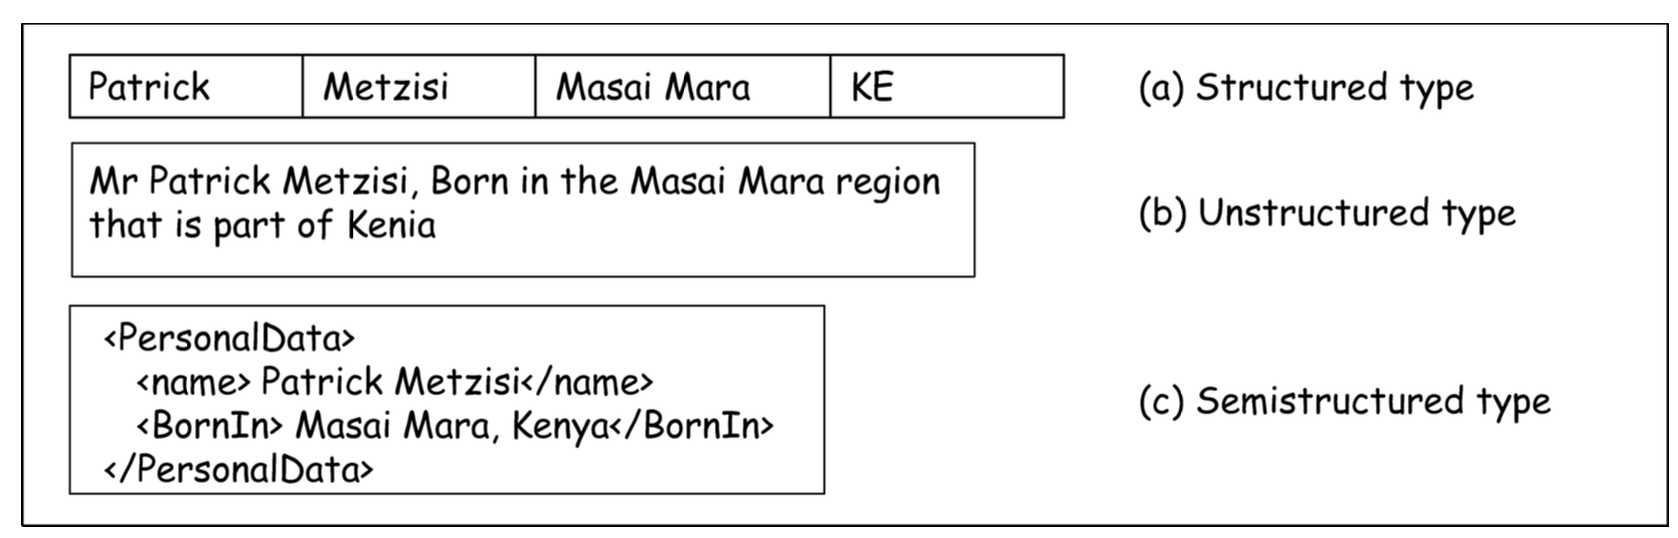
\includegraphics[width=1\textwidth]{Paper/figures/DataType.png}
        \caption{A circle (a) and a star (b). Note that any caption ends with a full stop character.}
        \label{fig:subfig}
    \end{figure}

    \subsection{Data Quality Problems}
    As the paper is aiming at classifying DQ assessment methods in the context of relational databases, this
    research focuses on the data perspective problems for both context dependent and independent categories and uses the classification of DQ problems identified in [5] (see Table 1).
    Hence, we provide a brief definition for each DQ problem in the context of our research in the following.
    In the context independent category, spelling errors, missing data, and incorrect values are self-explanatory DQ problems.
    Duplicate data problems occur when rows are duplicated or when schemas contain redundancies (that is, specify duplicate attributes in multiple databases).
    Data format problems occur when two or more semantically equivalent data values have different representations (this includes inconsistent and text formatting DQ problems).
    Syntax violation problems occur when a pre-specified format has been assigned to an attribute and a data value for this attribute does not adhere to this format (this includes the incomplete data format DQ problem in Table 1).
    Problems with violations of integrity constraints arise when data values do not adhere to pre-specified database integrity constraints; we also therefore include unique value violations, rather than have these as a separate problem, because unique value violations are one type of database integrity constraint.
    Note that, despite its position in Table 1, we treat outdated data to be a user perspective problem because whether data is out of date depends on the purpose it is used for.
    For the context dependent category, the problem of violation of domain constraints is when an attribute value must be in a pre-specified context-dependent domain of values.
    Violation of organizational business rules is when any set of values do not adhere to a pre-specified rules assigned by the organization.
    Violation of company and governmental regulations is when any set of values do not adhere to a prespecified rules assigned imposed on the organization by legislating bodies.
    Similarly, violation of constraints provided by the database administrator is when any set of values do not adhere to a pre-specified rules assigned by the database administrator.



    \section{Literature Review}
    In this section, 3~5 data quality assessment methods are introduced in brief:
    Total Data Quality Management(TDQM),
    Total Information Quality Management(TIQM),
    Data Quality Assessment(DQA),
    Information Quality Measurement(IQM),
    Comprehensive methodology for Data Quality management(CDQ).



    \subsection{Total Data Quality Management (TDQM)}

    The TDQM methodology was the first general methodology pub- lished in the data quality literature [Wang 1998]. TDQM is the outcome of academic research, but has been extensively used as a guide to organizational data reengineering initiatives. The fundamental objective of TDQM is to extend to data quality, the principles of Total Quality Management (TQM) [Oakland 1989].

    TQM has shifted the focus of reengineering activities from efficiency to effectiveness, by offering methodological guidelines aimed at eliminating discrepancies between the out- put of operating processes and customers’ requirements. Given requirements, reengineering must start from modeling operating processes. Consistent with these tenets, TDQM proposes a language for the description of information production (IP) processes, called IP-MAP [Shankaranarayan et al. 2000]. IP-MAP has been variously extended, towards UML and also to support organizational design. IP-MAP is the only language for information process modeling and represents a de facto standard. Practical experiences with TDQM are reported, for example, in Kovac and Weickert [2002].

    TDQM’s goal is to support the entire end-to-end quality improvement process, from requirements analysis to implementation.
    As shown in Figure 6(a) TDQM Cycle consists of four phases that implement a continuous quality improvement process: definition, measurement, analysis, and improvement.
    The roles responsible for the different phases of the quality improvement process are also defined in TDQM.
    Four roles are distinguished: information suppliers, which create or collect data for the IP, information manufacturers, which design, develop, or maintain data and related system infrastructure, information consumers, which use data in their work, and information process managers, which are responsible for managing the entire information production process throughout the information life cycle.
    TDQM is comprehensive also from an implementation perspective, as it provides guidelines as to how to apply the methodology.
    In applying TDQM, an organization must:
    (a) clearly understand the IPs;
    (b) establish an IP team consisting of a senior executive as the TDQM champion, an IP engineer who is familiar with the TDQM methodology, and members who are information suppliers, manufacturers, consumers, and IP managers;
    (c) teach IQ assessment and IQ management to all the IP constituencies; and
    (d) institutionalize continuous IP improvement.

    TDQM relies on the information quality literature for IQ Criteria and IQ improvement techniques.
    In particular, it explicitly refers to Wang and Strong [1996] for the data quality dimensions specification.
    TDQM relates quality issues to corresponding improvement techniques.
    However, in the recent literature no industry-specific technique is referred and no support is offered to specialize general quality improvement techniques.


    \subsection{Total Information Quality Management (TIQM)}

    The TIQM methodology [English 1999] has been designed to support data warehouse projects. The methodology assumes the consolidation of operational data sources into a unique, integrated database, used in all types of aggregations performed to build the data warehouse. This consolidation eliminates errors and heterogeneities of source databases. TIQM focuses on the management activities that are responsible for the integration of operational data sources, by discussing the strategy that has to be followed by the organization in order to make effective technical choices. Cost-benefit analyses are supported from a managerial perspective. The methodology provides a detailed classification of costs and benefits (see Section 3.4).

    Figure 8 shows the phases of the TIQM methodology.
    From the TIQM’s managerial perspective, there are three main phases: assessment, improvement, and improvement management and monitoring.
    One of the valuable contributions of the methodology is the definition of this last phase, which provides guidelines to manage changes in the organization’s structure according to data quality management requirements.
    Furthermore, the economics approach introduces cost benefit evaluation to justify data quality interventions.
    The goal is not only the achievement of higher data quality level, but to undertake improvement actions only if they are feasible; thus only if benefits are greater than costs.

    \subsection{Data Quality Assessment (DQA)}
    General description. The DQA methodology [Pipino et al. 2002] has been designed to provide the general principles guiding the definition of data quality metrics. In the literature, data quality metrics are mostly defined ad hoc to solve specific problems and thus, are dependent on the considered scenario. The DQA methodology is aimed at identifying the general quality measurement principles common to previous research.

    Detailed comments. The classification of metrics of the DQA methodology is summarized in Figure 12. The methodology makes a distinction between subjective and objective quality metrics. Subjective metrics measure the perceptions, needs, and experiences of the stakeholders. Objective metrics are then classified into task-independent and task-dependent. The first assess the quality of data without contextual knowledge of the application, while the second are defined for specific application contexts and include business rules, company and government regulations, and constraints provided by the database administration. Both metrics are divided into three classes: simple ratio, min or max value, and weighed average.


    \subsection{Information Quality Measurement (IQM)}
    The fundamental objective of the IQM methodology [Eppler and Mu ̈nzenmaier 2002] is to provide an information quality framework tailored to Web data.
    In particular, IQM helps the quality-based selection and personalization of the tools that support Webmasters in creating, managing, and maintaining Web sites.

    The IQM methodology provides guidelines to ensure that software tools evaluate all the fundamental information quality dimensions.
    The methodology provides two sets of guidelines: the information quality framework defining quality criteria, and the action plan explaining how to perform quality measurements.
    The main phases of IQM methodology are reported in Figure 13. The first phase defines the measurement plan.
    The information quality framework is defined as a list of relevant information quality criteria identified by interviewing the information stake- holders.
    The framework is the input for an information quality audit that associates the information quality criteria with the methods and tools that will be used in the measurement process.
    Some criteria require multiple measurement methods. The IQM methodology coordinates the application of multiple measurement methods.

    \subsection{Comprehensive methodology for Data Quality management (CDQ)}

    The CDQ methodology [Batini and Scannapieco 2006; Batini et al. 2008] is conceived to be at the same time complete, flexible, and simple to apply.
    Completeness is achieved by considering existing techniques and tools and integrating them in a framework that can work in both intra- and inter-organizational contexts, and can be applied to all types of data, structured, semistructured and unstructured.
    The methodology is flexible since it supports the user in the selection of the most suitable techniques and tools within each phase and in any context.
    Finally, CDQ is simple since it is organized in phases and each phase is characterized by a specific goal and set of techniques to apply.

    The CDQ methodology is innovative since it provides support to select the optimal quality improvement process that maximizes benefits within given budget limits.
    Second, it emphasizes the initial requirements elicitation phase. In fact, the other methodologies implicitly assume that contextual knowledge has been previously gathered and modelled.
    The focus is on how to reach total data quality without providing indications as to how to use contextual knowledge.
    A goal of CDQ is instead to obtain a quantitative assessment of the extent to which business processes are affected by bad information.

    Three main phases characterize the methodology: state reconstruction, assessment, and choice of the optimal improvement process (see Figure 20).
    In the first phase of the methodology, the relationships among organizational units, processes, services, and data are reconstructed.
    These relationships are modelled by using matrixes that describe which organizational units use data and their roles in the different business processes.
    Furthermore, in this phase, processes are described along with their contribution in the production of goods/services and the legal and organizational rules that discipline workflows.
    The second phase sets new target quality levels that are needed to improve process qualities, and evaluates corresponding costs and benefits.
    This phase locates the critical variables affected by poor quality. Since improvement activities are complex and costly, it is advisable to focus on the parts of the databases and data flows that raise major problems.
    Finally, the third phase consists of five steps and is aimed at the identification of the optimal improvement process: the sequence of activities that has the highest cost/effectiveness ratio.
    New target quality levels are set by considering costs and benefits. Different improvement activities can be performed to reach new quality targets.
    The methodology recommends the identification of all the data-driven and process-driven improvement techniques for the different databases affected by poor quality.
    A set of mutually consistent improvement techniques constitutes an improvement process.
    Finally, the most suitable improvement process is selected by performing a cost-benefit analysis.

    \section{Evaluation}
    In this section evaluation in terns of process, techniques, and performances are discussed across these methods.
    \section{Conclusion}
    This section summarizes all the topics in report.
    The conclusions of evaluation of different method are drew.
    From the best suitable methods, new ideas and customization are proposed to be adapted in the context of CI/CD application in software engineering.
    In the end, the future work of data quality assessment for CI/CD application are proposed.
    \bibliography{template}

\end{document}
